\chapter{T1 --- Modos lentos del Liouvilliano (Arnoldi--Lindblad)}
\label{ch:t1}

\ideacentral{Bajo el modelo de Ising disipativo, T1 valida que el algoritmo
Arnoldi--Lindblad extrae la \emph{estructura de relajación} del Liouvilliano
---los modos lentos $\lambda_2,\hat r_2,\hat l_2$ y los solapamientos $a_k$, que
\emph{predicen} si una preparación exhibe QMpE ($a_2\!\approx\!0$)--- a coste
\emph{matrix-free} paralelizable, con la precisión de la diagonalización exacta
($\text{error}\le10^{-5}$) y aceleración algorítmica \emph{faster-than-the-clock}
($8.8\times$). Es decir: el dato que \textbf{predice} el efecto se obtiene de
forma correcta y escalable ---prerequisito para verificarlo y explotarlo.}

\section{Marco teórico}

La tarea T1 consiste en extraer los autovalores de $\Lop$ más cercanos a $0$ ---el
estado estacionario $\lambda_1=0$ y los modos lentos $\lambda_2,\lambda_3,\dots$---
junto con sus autooperadores derecho $\hat r_k$ e izquierdo $\hat l_k$, que cumplen
\begin{equation}
    \Lop[\hat r_k]=\lambda_k\hat r_k, \qquad
    \Lop^\dagger[\hat l_k]=\lambda_k^*\hat l_k, \qquad
    \Tr(\hat l_j^\dagger \hat r_k)=\delta_{jk}.
\end{equation}
Con la base biortonormal se obtienen los solapamientos $a_k=\Tr(\hat l_k^\dagger\rho_0)$
de \cref{eq:spectral}; el criterio de Mpemba fuerte es $a_2=0$. No se necesita
todo el espectro: bastan los pocos $\lambda_k$ de parte real más próxima a cero,
que dominan la relajación a tiempos largos. Es un problema de \emph{autovalores
interior} con \emph{target} $\sigma=0$.

\section{Método numérico: Arnoldi sobre el propagador}

En lugar de diagonalizar $\Lop$ (denso, $\mathcal{O}(d^6)$) o de aplicar
\emph{shift-invert} $(\Lop-\sigma\mathbb{1})^{-1}$ (que exige resolver sistemas
lineales), seguimos el algoritmo \textbf{Arnoldi--Lindblad} de Minganti \&
Huybrechts (\emph{Quantum} \textbf{6}, 649, 2022). La idea es construir el
subespacio de Krylov del \emph{propagador}
\begin{equation}
    P(\tau) = e^{\tau\Lop},
\end{equation}
cuya acción $P(\tau)[V]$ se calcula \emph{matrix-free} integrando la ecuación
$\dot V = \Lop[V]$ en $[0,\tau]$ con RK4, usando el núcleo
\begin{equation}
    \Lop[V] = -i[H,V] + \sum_\mu\Big(L_\mu V L_\mu^\dagger
              - \tfrac12\{L_\mu^\dagger L_\mu, V\}\Big),
    \label{eq:spmv}
\end{equation}
sin materializar la matriz $d^2\times d^2$. El espectro de $P$ y el de $\Lop$ están
ligados por
\begin{equation}
    \mu_k = e^{\tau\lambda_k}, \qquad \lambda_k = \frac{\ln\mu_k}{\tau}.
\end{equation}
Como $\Re\lambda_k\le 0$, todos los $\mu_k$ caen en el disco unidad
$|\mu_k|\le 1$; el estacionario es $\mu_1=1$ y los \textbf{modos lentos} son los de
\emph{mayor módulo} $|\mu_k|$. La iteración de Arnoldi converge primero a los
autovalores dominantes en módulo de $P$ ---justamente los modos lentos de $\Lop$.
De ahí el carácter \emph{faster than the clock}: basta un subespacio de Krylov
pequeño (unas pocas acciones del propagador) en lugar de evolucionar el sistema
durante el tiempo físico $\tau_{\mathrm R}=1/|\Re\lambda_2|$.

\begin{algorithm}[t]
\caption{Arnoldi--Lindblad (extracción de modos lentos)}
\begin{algorithmic}[1]
\State \textbf{Entrada:} $H,\{L_\mu\}$, paso del propagador $\tau$, paso RK4 $dt$,
       dimensión de Krylov $m$, reinicios $R$, número de modos $k$
\State $V_0 \gets$ operador hermítico semilla;\quad $q_0 \gets V_0/\|V_0\|_{\mathrm{HS}}$
\For{$r=1,\dots,R$}
  \For{$j=0,\dots,m-1$}    \Comment{iteración de Arnoldi (Gram--Schmidt mod.)}
    \State $w \gets P(\tau)\,q_j = e^{\tau\Lop}[q_j]$  \Comment{RK4 matrix-free, \cref{eq:spmv}}
    \State $H_{ij}\gets\langle q_i,w\rangle_{\mathrm{HS}}$,\;
           $w\gets w-\sum_{i\le j}H_{ij}q_i$,\;
           $q_{j+1}\gets w/\|w\|$
  \EndFor
  \State $(\mu, Y)\gets\textsc{eig}(H_{m})$;\quad ordenar por $|\mu|$ desc.
  \State $\lambda_c \gets \ln(\mu_c)/\tau$;\quad $\hat r_c \gets \sum_i Y_{ic}\,q_i$
  \State \textbf{restart}: $V_0\gets\sum_{c\le k}\hat r_c$  \Comment{re-siembra con modos dominantes}
\EndFor
\State Repetir con $\Lop^\dagger$ para $\hat l_k$;\; biortonormalizar
\State \textbf{Salida:} $\{\lambda_k,\hat r_k,\hat l_k\}$, $\rss=\hat r_1/\Tr\hat r_1$
\end{algorithmic}
\end{algorithm}

El producto interno es el de Hilbert--Schmidt $\langle A,B\rangle_{\mathrm{HS}}=\Tr(A^\dagger B)$.
Los autooperadores izquierdos se obtienen repitiendo la iteración sobre el
Liouvilliano dual $\Lop^\dagger$ y biortonormalizando el pequeño conjunto
resultante.

\section{Implementación serial}

La referencia serial está en \texttt{T1/python/arnoldi\_lindblad.py} (numpy puro),
trabajando en el espacio de operadores $d\times d$ (formulación natural
matrix-free). La acción del propagador es:
\begin{lstlisting}[language=Python,caption={Accion del propagador exp(tau L)[V] por RK4, matrix-free (extracto).}]
def propagator_action(H, Ls, V, tau, dt, dual=False):
    apply = apply_liouvillian_dual if dual else qmpe.apply_liouvillian
    n_steps = max(1, int(np.ceil(tau / dt))); h = tau / n_steps
    X = V.astype(complex).copy()
    for _ in range(n_steps):
        k1 = apply(H, Ls, X);            k2 = apply(H, Ls, X + 0.5*h*k1)
        k3 = apply(H, Ls, X + 0.5*h*k2); k4 = apply(H, Ls, X + h*k3)
        X = X + h*(k1 + 2*k2 + 2*k3 + k4)/6.0
    return X
\end{lstlisting}

\section{Justificación de la paralelización}

La iteración de Arnoldi es \emph{secuencialmente acoplada}: cada vector de Krylov
$q_{j+1}$ depende de $q_j$ a través del propagador, y la ortogonalización
Gram--Schmidt encadena los productos internos. Por tanto, \textbf{el único
paralelismo escalable vive dentro del SpMV} \cref{eq:spmv}, que es el
\emph{hotspot} (el coste total es $n_{\mathrm{it}}\cdot\text{SpMV}$). El SpMV
matrix-free se reduce a productos de matrices densas $d\times d$, de coste
$\mathcal{O}(d^3)$. Adoptamos dos niveles:
\begin{itemize}
  \item \textbf{OpenMP} (intranodo): paraleliza el producto de matrices del SpMV
  sobre las filas.
  \item \textbf{MPI} (internodo): distribuye las filas de cada \texttt{matmul}
  entre rangos y reconstruye el resultado con \texttt{MPI\_Allgatherv}
  (paralelismo de datos, \S 8.1 nivel 1 del informe). Los productos internos de
  Arnoldi son reducciones globales redundantes (baratas, $\mathcal{O}(d^2)$).
\end{itemize}
El pequeño problema de autovalores del Hessenberg $m\times m$ se resuelve con
LAPACK (\texttt{zgeev}); es despreciable frente al SpMV.

La implementación está en \texttt{T1/cpp/} (\texttt{qmpe\_core.hpp},
\texttt{arnoldi\_lindblad\_mpi.cpp}), compilable con CMake (MPI + OpenMP + LAPACK).

\section{Comparación y resultados}

\subsection{Validación contra el oráculo denso}

La \cref{tab:t1val} compara los autovalores lentos obtenidos por Arnoldi--Lindblad
(serial Python) contra la diagonalización densa completa, sobre los modelos
resolubles del informe. El error en los modos lentos va de $10^{-13}$ a
$2.6\times10^{-5}$, y el estado estacionario se reproduce a $\sim 10^{-11}$. El
núcleo C++ reproduce el mismo $\lambda_2=-0.69558$ para Ising $N=4$ a 6 cifras.

\begin{table}[t]
\centering
\caption{T1: error de Arnoldi--Lindblad frente a la diagonalización densa, y
coste \emph{faster-than-the-clock} (SpMV para alcanzar el estacionario por
evolución directa frente a Arnoldi).}
\label{tab:t1val}
\begin{tabular}{lccccc}
\toprule
Modelo & $d$ & $\lambda_2$ (denso) & error $\lambda_{\text{lentos}}$ & SpMV evol. / Arnoldi & speedup \\
\midrule
TLS        & 2 & $-0.6565$ & $5\times10^{-13}$ & $23\,612 / 27\,648$ & $0.9\times$ \\
$\Lambda$-3 & 3 & $-0.0627$ & $7\times10^{-12}$ & $400\,000 / 45\,472$ & $\mathbf{8.8\times}$ \\
Ising $N{=}2$ & 4 & $-0.5825$ & $1\times10^{-11}$ & $43\,812 / 152\,000$ & $0.3\times$ \\
Ising $N{=}3$ & 8 & $-0.7231$ & $3\times10^{-5}$ & $41\,464 / 152\,640$ & $0.3\times$ \\
\bottomrule
\end{tabular}
\end{table}

El \emph{faster-than-the-clock} se manifiesta cuando la relajación es lenta: en el
sistema $\Lambda$ de tres niveles ($\lambda_2\approx-0.063$, tiempo de relajación
$\sim 16$), Arnoldi--Lindblad alcanza el estacionario con $8.8\times$ menos
aplicaciones del Liouvilliano que la evolución directa. En sistemas de relajación
rápida la evolución directa ya es barata y Arnoldi no aporta ventaja: un resultado
honesto, coherente con que el método brilla cuando hay separación de escalas
(\cref{fig:t1eigs}).

\begin{figure}[t]
\centering
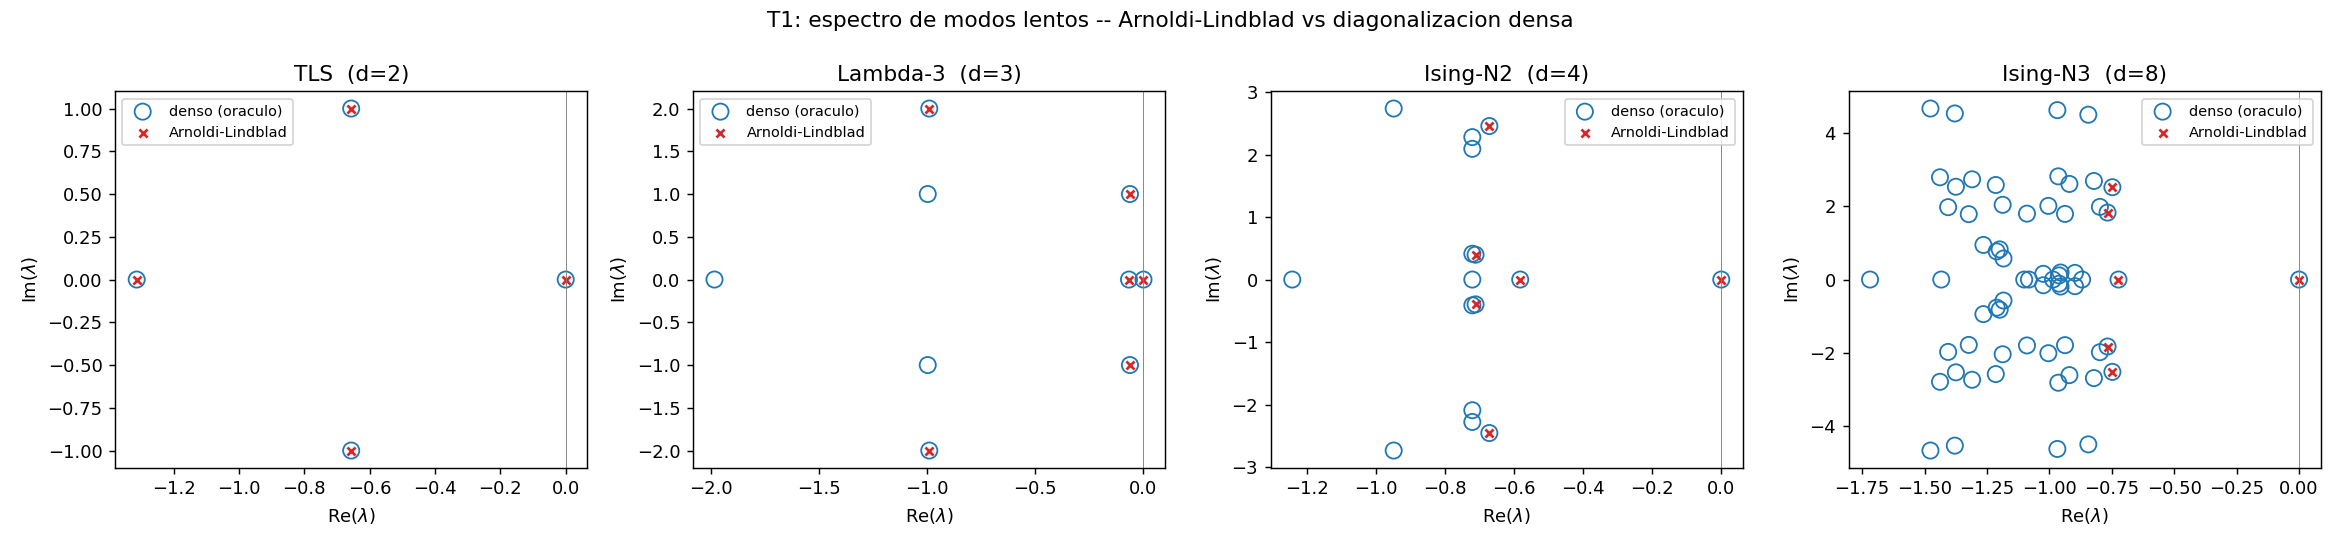
\includegraphics[width=\textwidth]{figures/t1_eigs.png}
\caption{Espectro de modos lentos: Arnoldi--Lindblad (cruces) frente a la
diagonalización densa (círculos) en el plano complejo, para los cuatro modelos.}
\label{fig:t1eigs}
\end{figure}

\subsection{Escalado paralelo}

La \cref{fig:t1scaling} y la \cref{tab:t1scaling} muestran el escalado del núcleo
C++ sobre Ising $N=7$ ($d=128$, $\dim\Lop=16\,384$). Tanto OpenMP como MPI escalan
de forma similar hasta $\sim 2.9\times$ con 4 \emph{workers}, con saturación a 8
por el ancho de banda de memoria (el \texttt{matmul} es \emph{memory-bound}). Es
notable que MPI escale prácticamente igual que OpenMP pese a la comunicación
\texttt{Allgatherv}: el cómputo $\mathcal{O}(d^3)$ amortiza el intercambio de
$\mathcal{O}(d^2)$ por \texttt{matmul}.

\begin{table}[h]
\centering
\caption{T1: speedup del SpMV distribuido (Ising $N=7$, $d=128$).}
\label{tab:t1scaling}
\begin{tabular}{cccc}
\toprule
workers & OpenMP & MPI \\
\midrule
2 & $1.79\times$ & $1.81\times$ \\
4 & $2.89\times$ & $2.71\times$ \\
8 & $2.95\times$ & --- \\
\bottomrule
\end{tabular}
\end{table}

\begin{figure}[t]
\centering
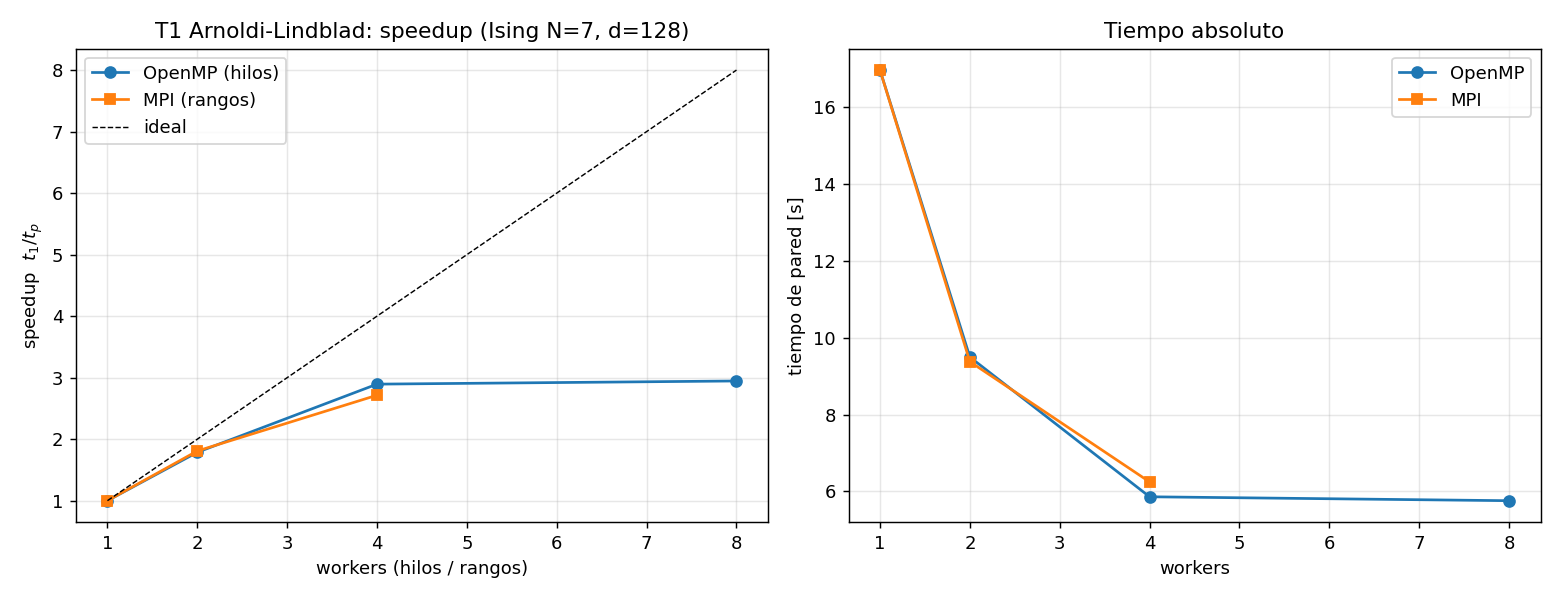
\includegraphics[width=\textwidth]{figures/t1_scaling.png}
\caption{Escalado de T1 (Arnoldi--Lindblad, Ising $N=7$): speedup y tiempo de
pared frente al número de hilos (OpenMP) y rangos (MPI).}
\label{fig:t1scaling}
\end{figure}

\medskip
\noindent\textbf{Limitación y trabajo futuro.} La distribución MPI reparte el
\emph{cómputo} del \texttt{matmul} pero mantiene los operadores replicados (la
memoria no se distribuye). El escalado real a muchos cuerpos requiere
almacenamiento disperso (CSR) de $H$ y $L_\mu$, que aprovecha que el SpMV preserva
la dispersión ($\mathcal{O}(d^2\,\mathrm{poly}\,N)$ no nulos) ---la costura de
paralelización señalada en el informe.
